
\chapter{Manual de uso}
\label{Appendix:Key2}

En este apéndice se explicará brevemente cómo usar las distintas funcionalidades de la herramienta, aportando imágenes de la terminal o de la herramienta para facilitar su entendimiento.

\section{Ejemplos de Ejecución}

El archivo ``script\_ejecucion.py'' y ``launch.py'' es ejecutable de la manera estándar de Linux, $./archivo$ o con $python3$.\\

El mensaje de ayuda generado por la herramienta al ejecutar ``script\_ejecucion.py'' con la opción -h o --help es:


\begin{minted}{bash}
Usage: script_ejecucion.py [OPTIONS] COMMAND [ARGS]...

  Herramienta para la ocultacion y desocultacion de datos en imagen y
  audio.

Options:
  -h, --help  Show this message and exit.

Commands:
  desocultar  Ejecuta la acción de desocultación.
  ocultar     Ejecuta la acción de ocultación.
\end{minted}

y ejecutando cada subcomando con la misma opción:

\begin{minted}{bash}
> ./script_ejecucion.py ocultar -h
Usage: script_ejecucion.py ocultar [OPTIONS]

  Ejecuta la acción de ocultación.

Options:
  --modo-cifrado [aes|none]       Modo de cifrado a utilizar.
  --modo-cifrado-imagen [lsb|text]
                                  Modo de ocultacion a usar en la imagen.
  --modo-cifrado-audio [lsb|sstv]
                                  Modo de ocultacion específico para audio.
  -v, --verbose                   Modo verbose , muestra mensajes del
                                  flujo.
  -i, --input PATH                Archivo de datos a ocultar  [required]
  --input_imagen PATH             Archivo de imagen requerido para ciertos
                                  modo de ocultacion de imagen.
  --input_audio PATH              Archivo de audio requerido para ciertos
                                  modo de ocultacion de audio.
  -o, --output PATH               Nombre del archivo de salida.
  --contraseña TEXT               Contraseña para cifrado o descifrado.
  -h, --help                      Show this message and exit.
\end{minted}

\begin{minted}{bash}
> ./script_ejecucion.py desocultar -h
Usage: script_ejecucion.py desocultar [OPTIONS]

  Ejecuta la acción de desocultación.

Options:
  --modo-cifrado [aes|none]       Modo de cifrado a utilizar.
  --modo-cifrado-imagen [lsb|text|none]
                                  Modo de ocultacion usado en la imagen.
  --modo-cifrado-audio [lsb|sstv|none]
                                  Modo de ocultacion usado en el audio.
  -v, --verbose                   Modo verbose , muestra mensajes del
                                  flujo.
  -s, --streaming                 Modo streaming, captura el audio sstv en
                                  streaming en vez de pasarle un audio.
  --input_audio PATH              Archivo de audio de entrada.
  --input_imagen PATH             Archivo de imagen de entrada.
  -i, --input_text PATH           Archivo de texto de entrada.
  -o, --output PATH               Archivo de texto de salida.
  --contraseña TEXT               Contraseña para descifrado.
  -h, --help                      Show this message and exit.
\end{minted}

Para ejecutar la CLI $ python3\ launch.py$, este comando es lo que se ejecuta tras haber ejecutado el ``install.sh'' y ejecutar $pitea$ como se muestra en el apéndice \ref{Appendix:Key1}.

\subsection{Uso de algoritmos de ocultación basados en LSB}
\subsubsection{Llamada por terminal}
\begin{minted}{bash}
python3 script_ejecucion.py ocultar \
  --modo-cifrado aes \
  --modo-cifrado-imagen lsb \
  --modo-cifrado-audio lsb \
  -i archivos_prueba/prueba.txt \
  --input_imagen archivos_prueba/imagen.png \
  --input_audio archivos_prueba/audio.wav \
  -o ./archivos_prueba/audio_salida.wav \
  --contraseña qwqwqw \
  -v
\end{minted}

\begin{minted}{bash}
python3 script_ejecucion.py desocultar \
  --modo-cifrado aes \
  --modo-cifrado-imagen lsb \
  --modo-cifrado-audio lsb \
  --input_audio ./archivos_prueba/audio_salida.wav \
  -o ./archivos_prueba/datos_desocultos.txt \
  --contraseña qwqwqw \
  -v
\end{minted}
\newpage
\subsubsection{Llamada en la CLI}

\begin{figure}[h]
	\centering
	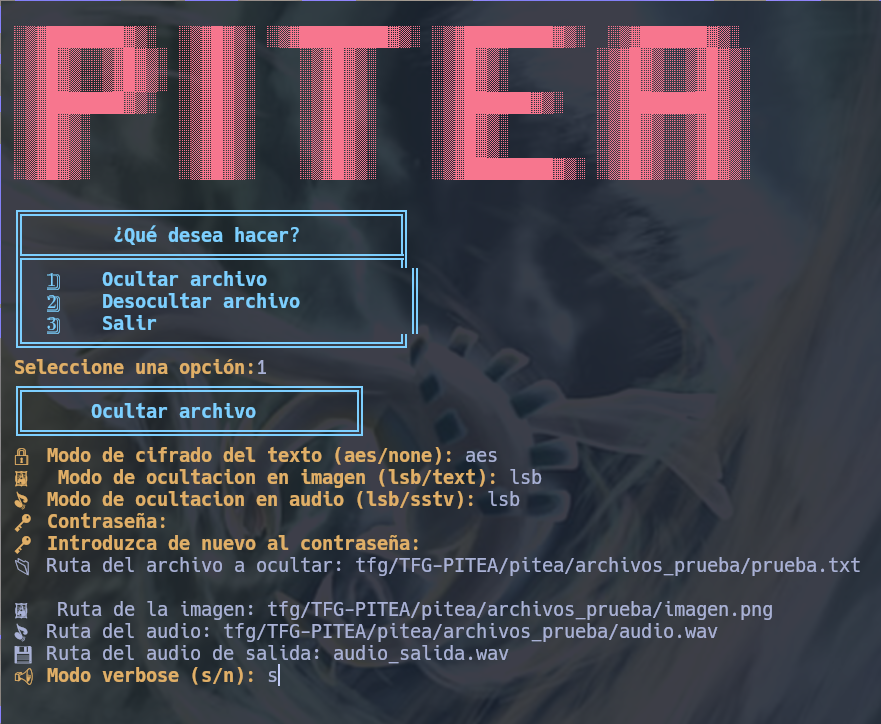
\includegraphics[width = 0.6\textwidth]{Imagenes/C/o_lsb.png}
	\caption[Ocultación LSB.]{Ejemplo de uso de la CLI para ocultación con LSB. Captura de pantalla de la herramienta.}
	\label{fig:proceso2}
\end{figure}

\begin{figure}[h]
	\centering
	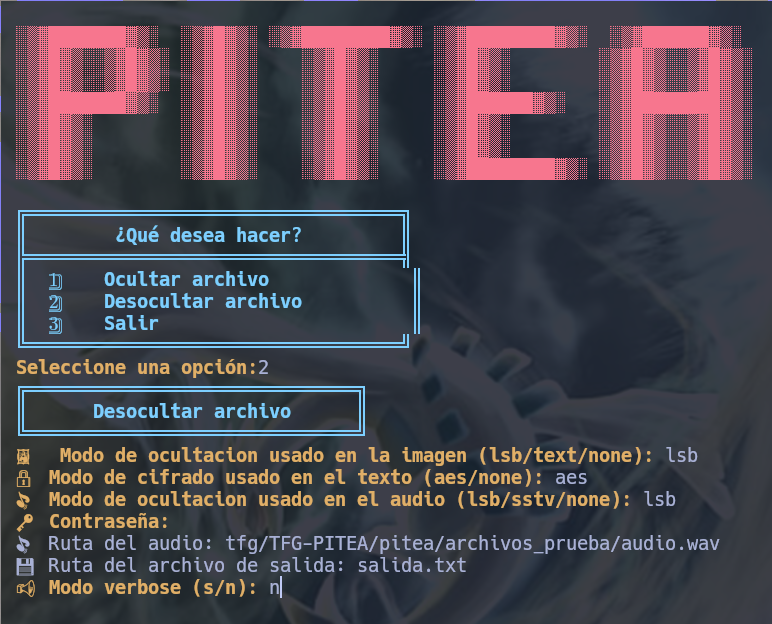
\includegraphics[width = 0.6\textwidth]{Imagenes/C/d_lsb.png}
	\caption[Descultación LSB.]{Ejemplo de uso de la CLI para desocultación con LSB. Captura de pantalla de la herramienta.}
	\label{fig:proceso2}
\end{figure}

\newpage
\FloatBarrier
\subsection{SSTV}

\begin{minted}{bash}
python3 script_ejecucion.py ocultar \
  --modo-cifrado aes \
  --modo-cifrado-imagen text \
  --modo-cifrado-audio sstv \
  -i archivos_prueba/prueba.txt \
  -o ./archivos_prueba/sstv.wav \
  --contraseña qwqwqw \
  -v
\end{minted}

\begin{figure}[h]
	\centering
	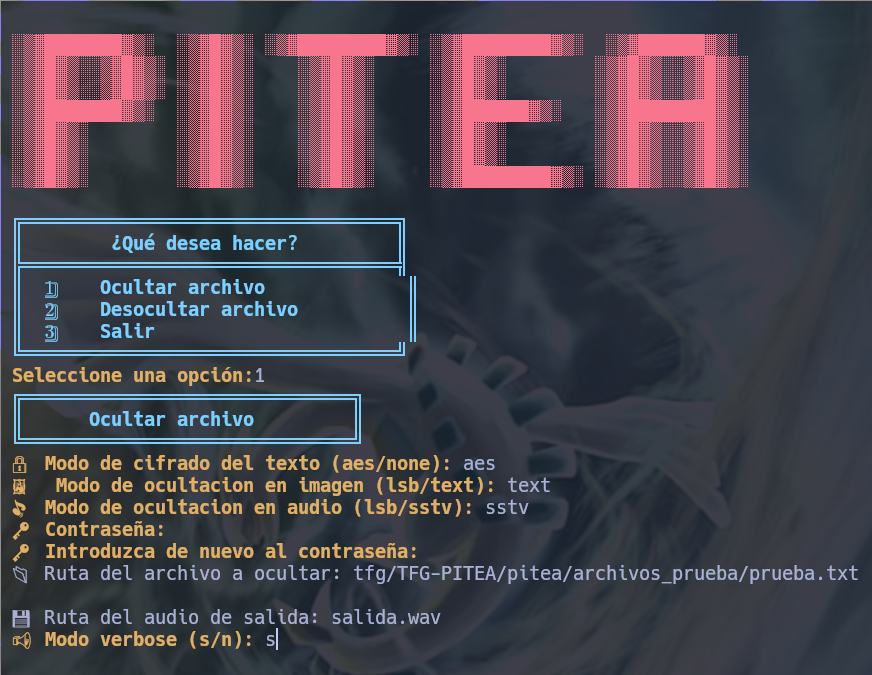
\includegraphics[width = 0.5\textwidth]{Imagenes/C/o_sstv.png}
	\caption[Ocultación SSTV.]{Ejemplo de uso de la CLI para ocultación con SSTV. Captura de pantalla de la herramienta.}
	\label{fig:proceso2}
\end{figure}

Para la desocultación de esta subsección es necesario configurar QSSTV. Es marcar la casilla del \textit{autoslant}.

\begin{figure}[h]
	\centering
	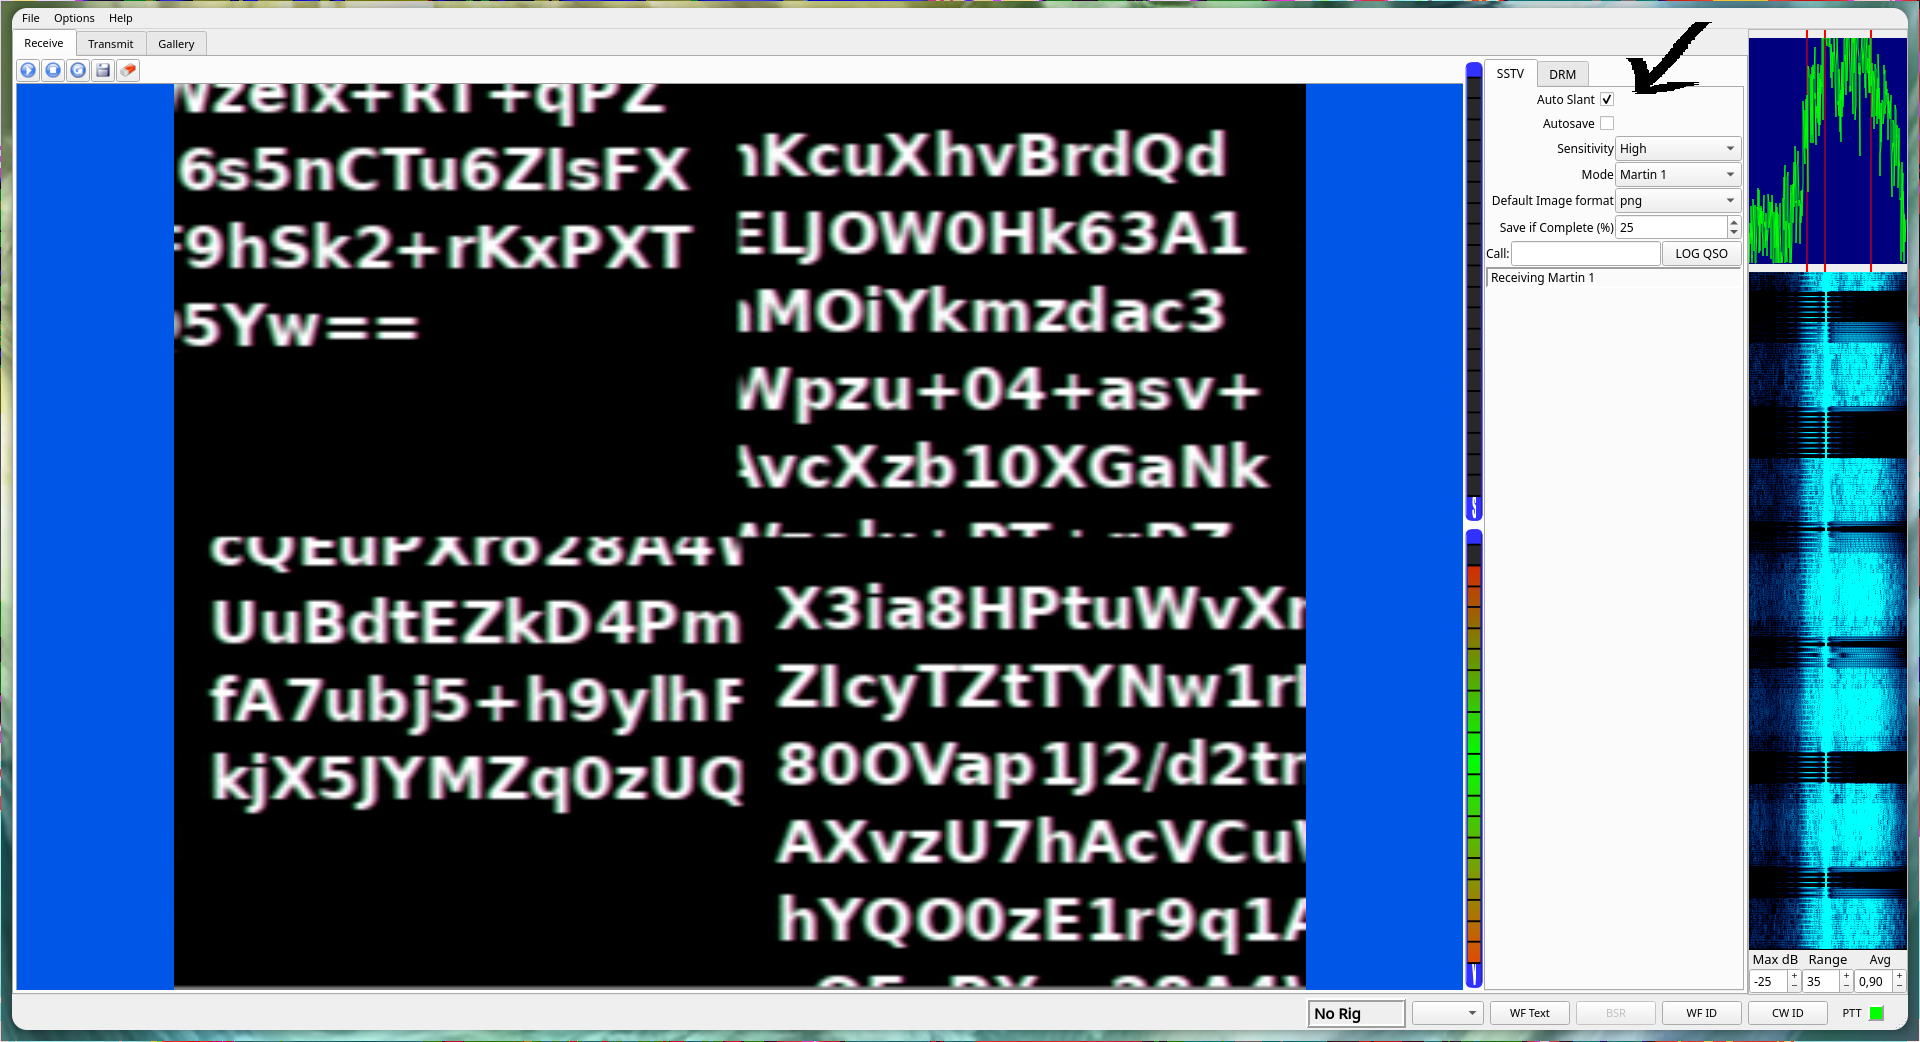
\includegraphics[width = 0.6\textwidth]{Imagenes/C/autoslant.png}
	\caption[Marcar \textit{autoslant}.]{Marcar \textit{autoslant}. Captura de pantalla de QSSTV.}
	\label{fig:proceso2}
\end{figure}

\subsubsection{Desocultación desde imagen}



\begin{minted}{bash}
python3 script_ejecucion.py desocultar \
  --modo-cifrado aes \
  --modo-cifrado-imagen text \
  --modo-cifrado-audio none \
  --input_imagen ./archivos_prueba/imagen_salida_sstv.png \
  -o ./archivos_prueba/datos_desocultos_text_sstv.txt \
  --contraseña qwqwqw \
  -v
\end{minted}

\begin{figure}[h]
	\centering
	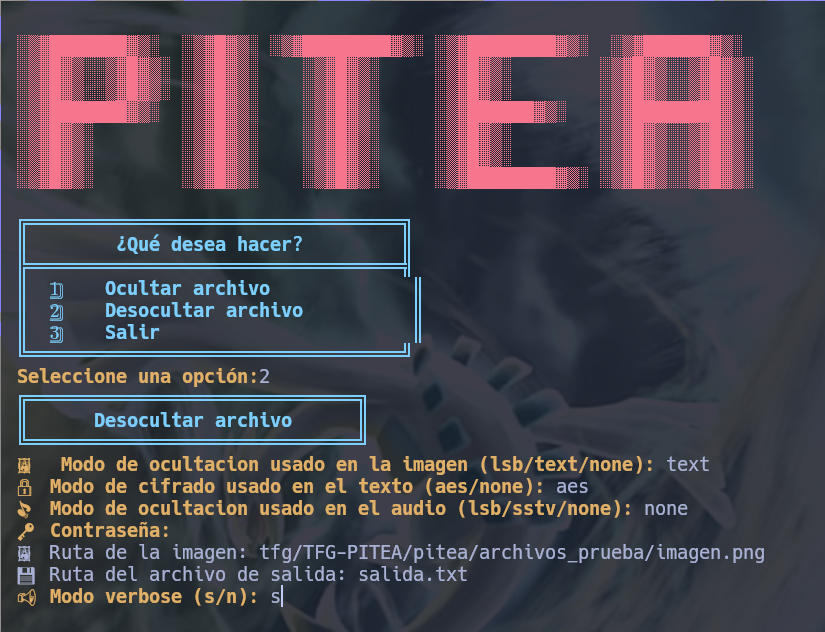
\includegraphics[width = 0.5\textwidth]{Imagenes/C/d_i_sstv.png}
	\caption[Descultación SSTV iniciando con una imagen.]{Ejemplo de uso de la CLI para desocultación con SSTV usando una imagen ya decodificada de SSTV. Captura de pantalla de la herramienta.}
	\label{fig:proceso2}
\end{figure}

\subsubsection{Desocultación desde audio}

Es necesario configurar QSSTV para que reciba el audio desde un archivo.

\begin{figure}[h]
	\centering
	
\includegraphics[width = 1\textwidth]{Imagenes/C/conf_file.png}
	\caption[Configuración QSSTV para archivos.]{Configuración QSSTV para lectura desde archivos. Capturas de pantalla de QSSTV.}
	\label{fig:proceso2}
\end{figure}
\newpage

\begin{minted}{bash}
python3 script_ejecucion.py desocultar \
  --modo-cifrado aes \
  --modo-cifrado-imagen text \
  --modo-cifrado-audio sstv \
  --input_audio ./archivos_prueba/sstv.wav \
  -o ./archivos_prueba/datos_desocultos_text_sstv.txt \
  --contraseña qwqwqw \
  -v
\end{minted}

\begin{figure}[h]
	\centering
	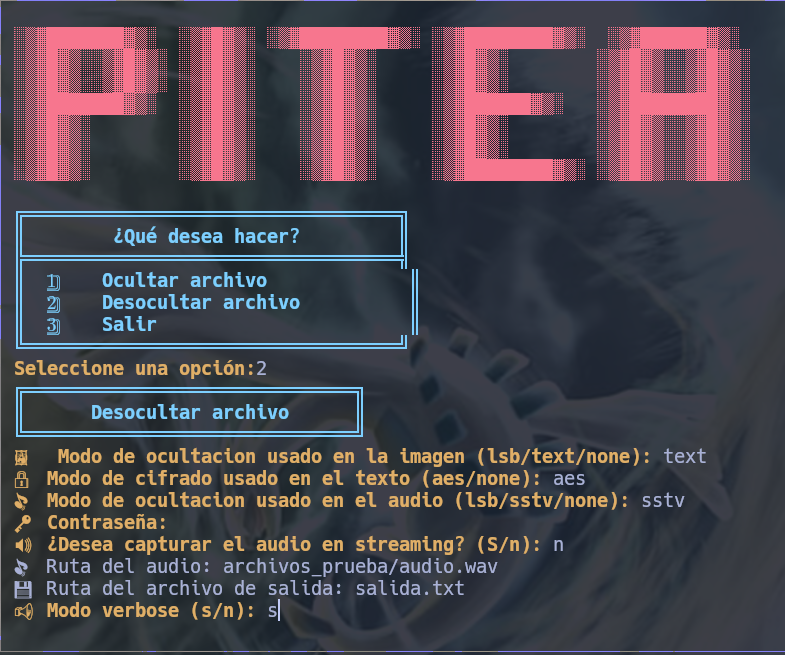
\includegraphics[width = 0.5\textwidth]{Imagenes/C/d_sstv.png}
	\caption[Descultación SSTV.]{Ejemplo de uso de la CLI para desocultación con SSTV. Captura de pantalla de la herramienta.}
	\label{fig:proceso2}
\end{figure}
\FloatBarrier



\subsubsection{Desocultación desde audio streaming}

Es necesario configurar QSSTV para que reciba el audio desde la tarjeta de sonido del dispositivo.

\begin{figure}[h]
	\centering
	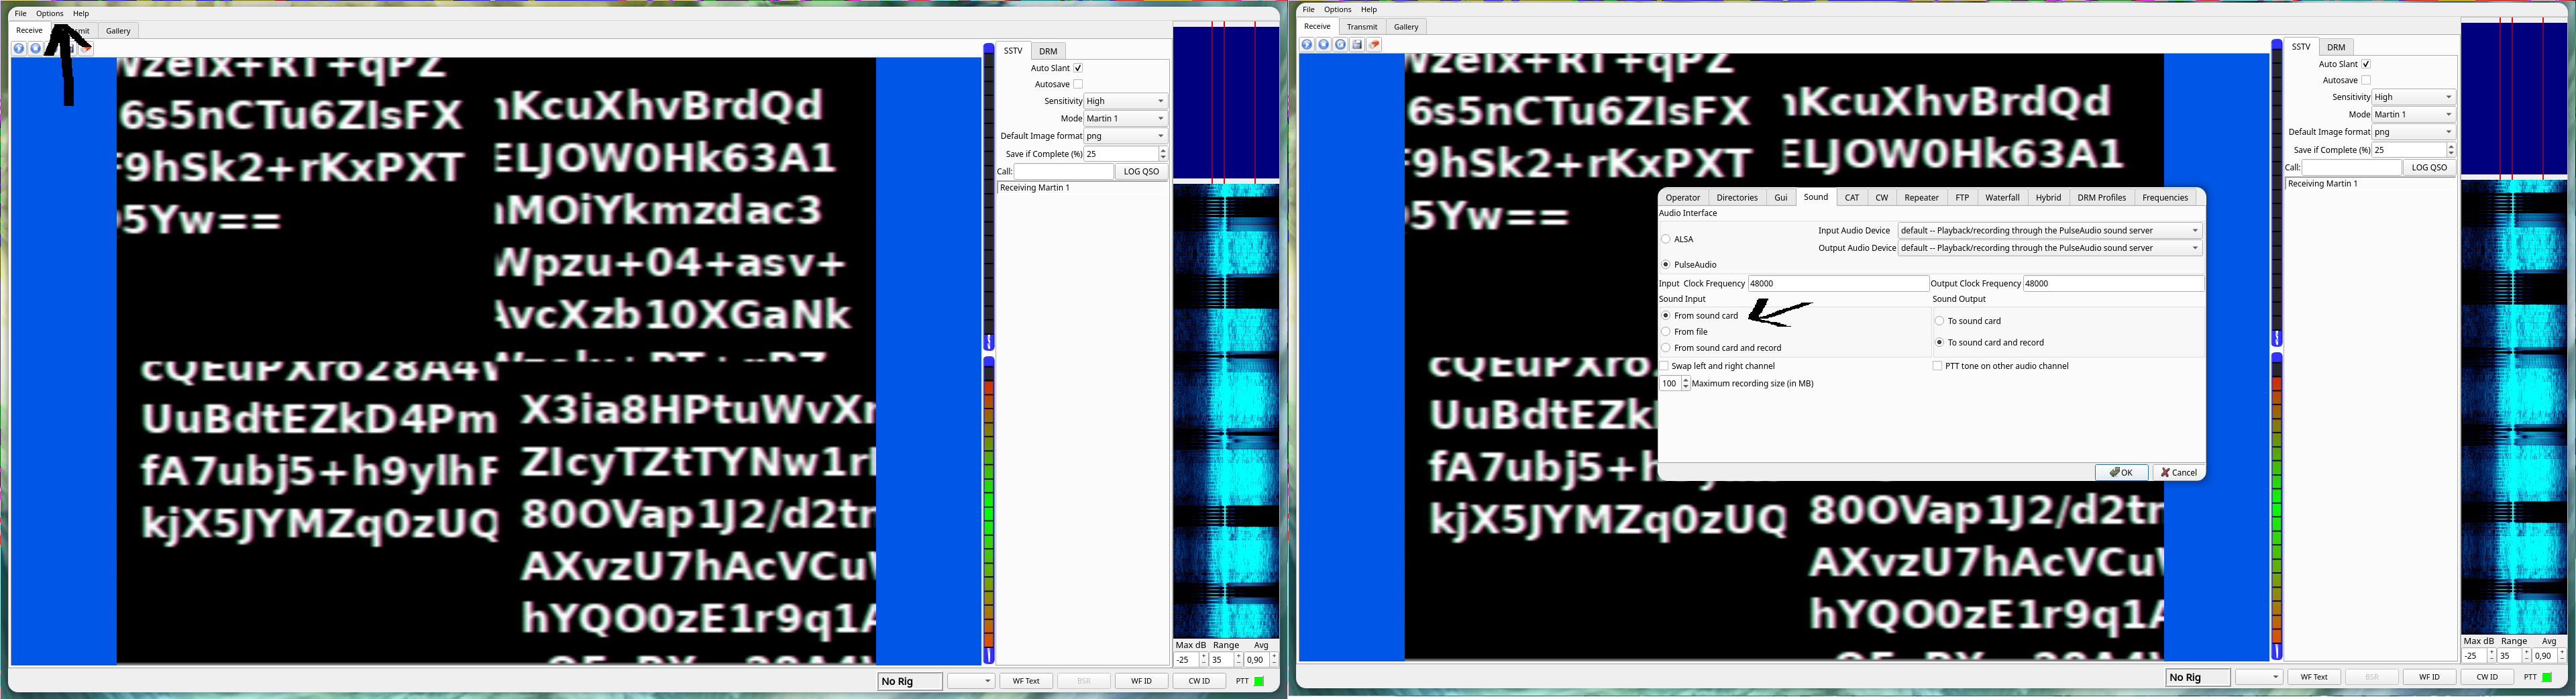
\includegraphics[width = 1\textwidth]{Imagenes/C/conf_sound.png}
	\caption[Configuración QSSTV para \textit{streaming}.]{Configuración QSSTV para lectura desde la tarjeta de sonido. Capturas de pantalla de QSSTV.}
	\label{fig:proceso2}
\end{figure}

\begin{minted}{bash}
python3 script_ejecucion.py desocultar \
  --modo-cifrado aes \
  --modo-cifrado-imagen text \
  --modo-cifrado-audio sstv \
  -o ./archivos_prueba/datos_desocultos_text_sstv.txt \
  --contraseña qwqwqw \
  -v \
  -s
\end{minted}

\begin{figure}[h]
	\centering
	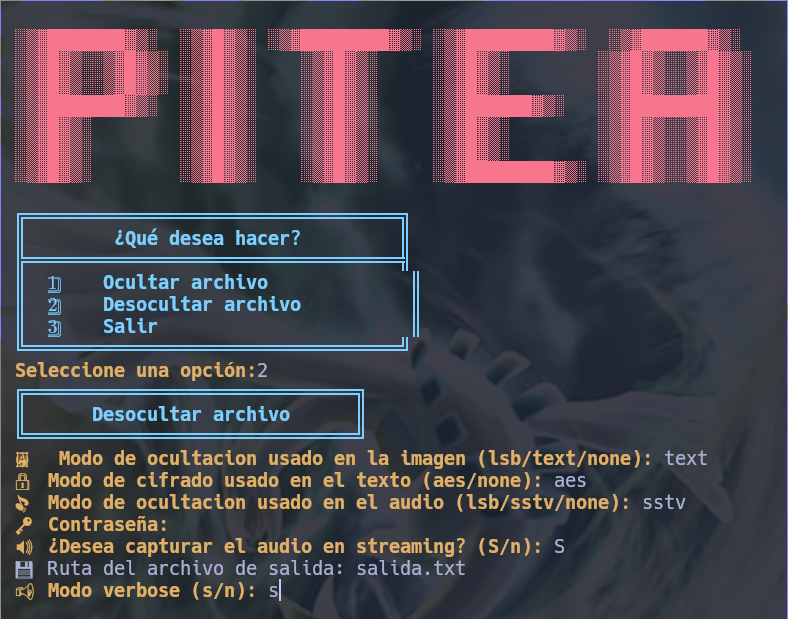
\includegraphics[width = 0.5\textwidth]{Imagenes/C/d_s_sstv.png}
	\caption[Descultación SSTV en modo \textit{streaming}.]{Ejemplo de uso de la CLI para desocultación con SSTV en modo \textit{streaming}. Captura de pantalla de la herramienta.}
	\label{fig:proceso2}
\end{figure}
\FloatBarrier

\subsubsection{Desocultación desde Base64}

\begin{minted}{bash}
python3 script_ejecucion.py desocultar \
  --modo-cifrado aes \
  --modo-cifrado-imagen none \
  --modo-cifrado-audio none \
  --input_text ./archivos_prueba/base64.txt \
  -o ./archivos_prueba/datos_desocultos_text_sstv.txt \
  --contraseña qwqwqw \
  -v
\end{minted}

\begin{figure}[h]
	\centering
	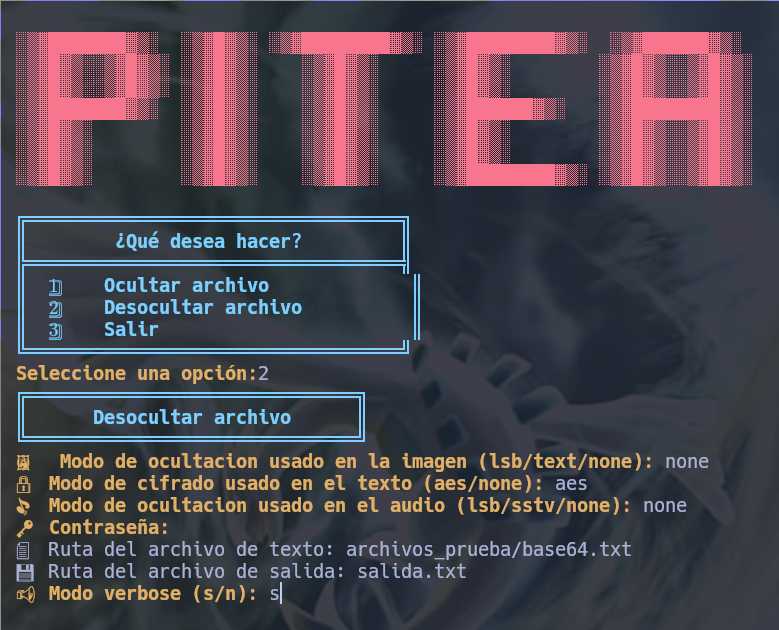
\includegraphics[width = 0.5\textwidth]{Imagenes/C/d_64_sstv.png}
	\caption[Descultación SSTV iniciando con un archivo que contiene base64.]{Ejemplo de uso de la CLI para desocultación con SSTV iniciando con un archivo que contiene información en base64. Captura de pantalla de la herramienta.}
	\label{fig:proceso2}
\end{figure}
\FloatBarrier

\section{Documentación del archivo de configuración, ``configuracion.toml''}


\begin{minted}[fontsize=\small, frame=lines, breaklines]{toml}
[persistente]
# Contador utilizado para distinguir la caché entre varias ejecuciones en un mismo minuto
contador_cache = 0

# Fecha de la última ejecución, usada para saber si es necesario utilizar el contador de caché
ult_fecha = "20-02-2025_21:22"

[Ajustes_sstv]
# Modo de transmisión SSTV seleccionado, especifica el tipo de imagen que se usará
modo_sstv = "MartinM1"

# Muestras por segundo, define la calidad de la transmisión en términos de frecuencia
samples_per_sec = 48000

# Número de bits por muestra, determina la resolución de las muestras de audio
bits = 16

[Ajustes_ocultador_imagen_text]
# Tamaño de la fuente en píxeles, utilizado para ajustar el texto sobre las imágenes
tamanio_fuente = 10

# Ancho máximo de las imágenes, para asegurarse de que las imágenes no sean demasiado anchas
anchura_maxima = 800

# Ruta relativa a la fuente utilizada para el texto (debe estar en el directorio adecuado)
ruta_fuente = "../fuentes/ocraregular.ttf"

# Configuración para usar la GPU, puede ser un valor booleano (True o False)
gpu = "True"
\end{minted}

\subsection*{Descripción de las secciones}

\begin{itemize}
    \item \texttt{persistente}: Guarda parámetros que se mantienen entre ejecuciones, como la caché y la fecha de la última ejecución.
    \item \texttt{Ajustes\_sstv}: Define la configuración de transmisión SSTV, incluyendo modo, muestras por segundo y resolución.
    \item \texttt{Ajustes\_ocultador\_imagen\_text}: Contiene opciones para superponer texto en imágenes, como tamaño de fuente, ancho máximo, fuente y uso de GPU.
\end{itemize}


